\chapter{Methoden}
\label{methods}
In diesem Kapitel wird aufgezeigt, wie die im Kapitel Einführung genannten Fragestellungen untersucht wurden.\\\\
Der Kern dieser Arbeit dreht sich um die folgende Frage: Verbessert sich ein CNN für eine spezifische Domäne, durch das hinzufügen domänenfremder Daten?
Konkret geht es darum, ob man annotierte domänenfremde Daten hinzuziehen kann, um ein CNN zu verbessern. Diese Fragestellung ist deshalb von Bedeutung, da es tendenziell immer zu wenig annotierte Daten gibt.
\section{Systemparameter}
\subsection{Hyperparameter}
\fixme{Hyperparametern}
\subsection{classweights}
Während der Anfangsphase dieser Arbeit wurde der Einfluss von classweights getestet. Die Ergebnisse zeigten eindeutig, dass die Perfomanz des CNN mit classweights steigt. Aus diesem Grund wird für alle weiteren Experimente immer mit classweights gearbeitet.\\\\
Dabei geht es um folgendes, in den Trainingsdaten sind die positiven, negativen und neutralen Sätze ungleich häufig verteilt. Dies würde in einem ungleichen Training für die entsprechenden Sentiments resultieren. Deshalb wird nun die Lernrate bei weniger häufig vorkommenden Sentiments verstärkt und bei denjenigen die überproportional vertreten sind, abgeschwächt.
\fixme{First draft classweights}
\subsection{EarlyStopping}
\fixme{EarlyStopping}
\subsection{$F1_{pn}$ Score}
Um die Ergebnisse der Experimente zu vergleichen, wurde der positive und negative gemittelte $F1_{pn}$ Score gewählt. 
Der $F1_{pn}$ Score wird folgendermassen berechnet:\\
\begin{equation}
F1_{p|n} = 2*\frac{precission*recall}{precission+recalll}
\end{equation}\\
Der F1 Score wird für die positiven, wie auch die negativen Fälle berechnet und dann wie folgt gemittelt:\\
\begin{equation}
F1_{pn} = \frac{F1_p+F1_n}{2}
\end{equation}\\
Dieser Wert gilt als Standart um die Qualität einer binärer \fixme{positiv, neutral und negativ kann auf ein binäres Klassifizierungsproblem zurückgeführt werden} Klassifizierung zu messen. Der grosse Vorteil dieses Masses ist, dass durch eine einseitige, falsche Klassifizierung, der Wert sehr schlecht wird.
\fixme{Beispiel hinzufügen, weshalb F1 Score gut ist}
\section{Word-Embeddings und Distant-Phase}
\subsection{Word-Embeddings}
Alle Experimente wurden mit 2 verschiedenen Word-Embeddings durchgeführt. Dabei soll der Einfluss, vielleicht auch eine Korrelation, zwischen den gewählten Word-Embedings und der Zieldomäne untersucht werden. Die Experimente wurden mit SemEval\_tweets und MPQ\_news Embeddings durchgeführt. Dass Tweets häufig aus vielen kurzen, teilweise auch stark abgekürzte Sätzen bestehen und News aus längeren, grammatikalisch korrekten Sätzen, wurde absichtlich so gewählt, damit allfällige Unterschiede im Resultat deutlicher sichtbar werden.
\subsection{Distant-Phase}
Aus der Arbeit \cite{deriu2016sentiment} ist ersichtlich, dass dieser Vorgang mit Tweets eine Verbesserung von fast 5 Prozentpunkte auf den $F1_{pn}$ Score erbrachte.
Deshalb wurde in dieser Arbeit eine Distant-Phase mit Amazon\_reviews Daten getestet. Wie im Kapitel Distant Supervision beschriben, muss aufgrund einer Eigenschaft der Daten ein Sentiment abgeleitet werden. Dabei bietet sich bei Reviews die Anzahl Sterne an, die vergeben wurden. Die Grenzen zwischen positiv/neutral und neutral/negativ sind nicht scharf und somit Definitionssache. In dieser Arbeit wurde folgende Definition angewendet: 1-2 Sterne für ein negatives Review, 3 Sterne für ein neutrales Review und 4-5 Sterne für ein positives review.
Alle nachfolgend beschrieben Experimente wurden einmal mit und einmal ohne einer Distanz-Phase durchgeführt.

\section{Aufbau der Experimente}
\label{experiments}
Die folgenden Experimente wurden jeweils für die Zieldomäne SemEval Tweets und MPQ Reviews durchgeführt. Bei allen Experimenten wird das CNN mit den gleichen Parametern initialisiert.
\subsection{Namensgebung der Experimente}
Die 3 Experimente CrossDomain, SimilarDomain und BaseDomain wurden mit den zwei Zieldomänen MPQ\_news und SemEval\_tweets jeweils durchgeführt, zusätzlich wurden alle Experimente mit beiden Embeddings getestet und schlussendlich wurden alle Experimente einmal mit einer Distant-Phase und einmal ohne eine Distant-Phase ausgeführt. Da dies eine grosse Menge an Resultate liefert, ist nachfolgend die Namensgebung geregelt:

\begin{enumerate}  
	\item Wort - Gibt an welches der 3 Experimenttypen gemeint ist. (CD = CrossDomain $\vert$ SD = SimilarDomain $\vert$ BD = BaseDomain)
	\item Wort - definiert die Zieldomäne (news = MPQ\_news $\vert$ tweets = SemEval\_tweets)
	\item Wort - steht für die gewählten Embeddings (newsEmb $\vert$ tweetEemb)
	\item Wort - gibt an, ob das Experiment mit oder ohne der Distant-Phase auf Amazon\_reviews ausgeführt wurde (withDP $\vert$ withoutDP)
	\item Wort - Wenn es sich um  ein einzelnes Experiment handelt, so steht am Ende des Namens die entsprechende Prozentzahl. Wenn keine Prozentzahl angegeben wird, so sind alle Experimente der entsprechenden Versuchsreihe gemeint.
\end{enumerate}
Getrennt werden die einzelnen Wörter Angaben mit einem Unterstrich. Nachfolgend zwei Beispiele:
\begin{itemize}  
	\item CrossDomain\_news\_newsEmb\_withDP
	\item SimilarDomain\_tweets\_tweetsEmb\_withoutDP-200
\end{itemize}
Beim ersten Beispiel sind alle Experimente der Reihe CrossDomain, mit der Zieldomäne MPQ\_news, mit news Embeddings und einer Distant-Phase, von 0-200 Prozent gemeint. Das zweite Beispiel ist analog dem Ersten zu interpretieren, mit der Besonderheit, dass nur ein Experiment (dasjenige mit 200$\%$ Zieldomäne Daten) gemeint ist.
\subsection{Experiment CrossDomain}
Mit dem Experiment V6 wurde die Kernfrage untersucht, ob die Performanz eines CNN steigt, wenn Domänenfremde Daten in die Trainingsphase mit einbezogen werden.
In einem ersten Schritt wurde das CNN mit domänenfremden Daten trainiert. Anschliessend wird das CNN in 21 Einzelschritten mit jeweils zusätzlich 400 Daten von der Zieldomäne weiter trainiert. Die genaue Aufteilung auf die verschiedenen Domänen ist im Bild \ref{fig:Method_CrossDomain} ersichtlich.
\begin{figure}[H]
	\centering
	\subfigure[Zieldomäne MPQ\_news]{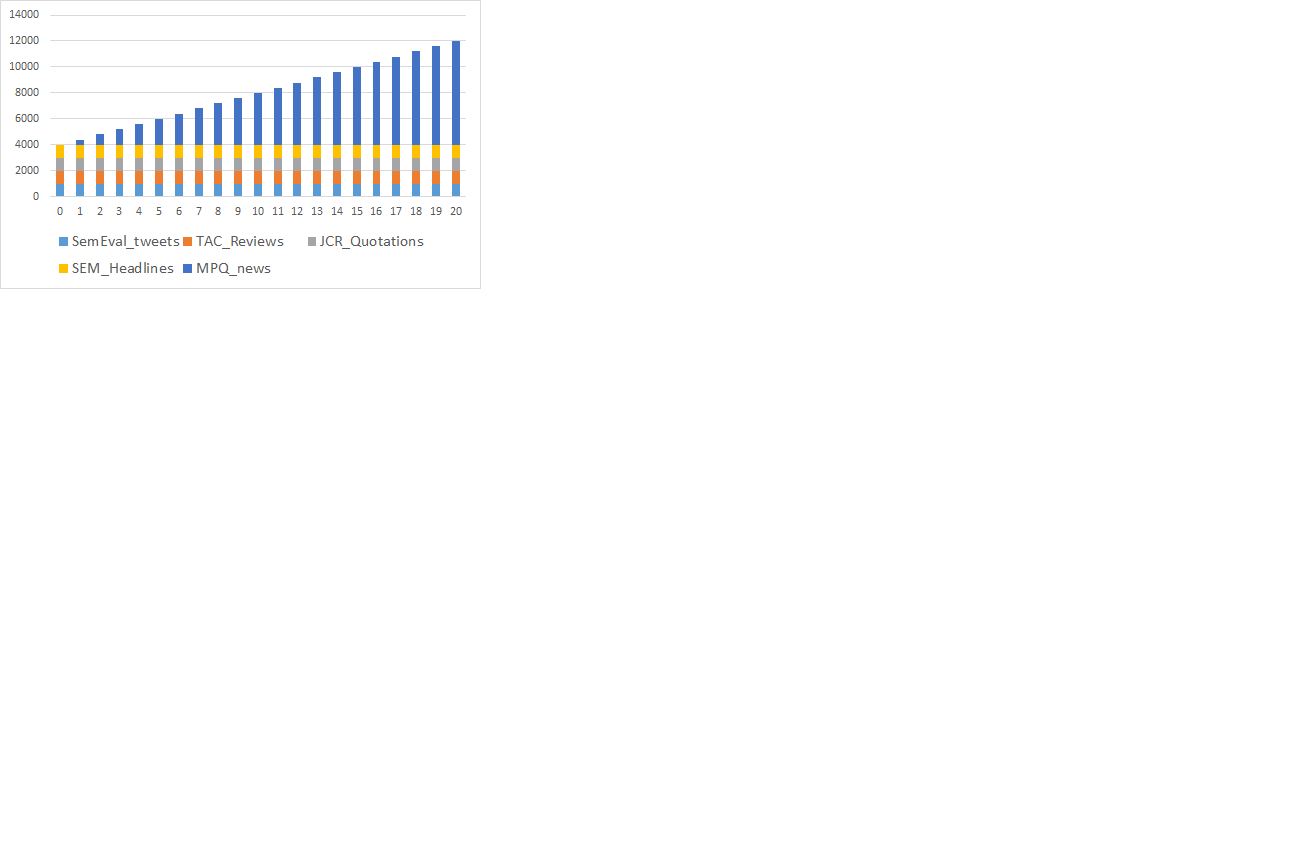
\includegraphics[width=0.49\textwidth]{img/methods/config_CrossDomain_MPQ_news.PNG}}
	\subfigure[Zieldomäne SemEval\_tweets]{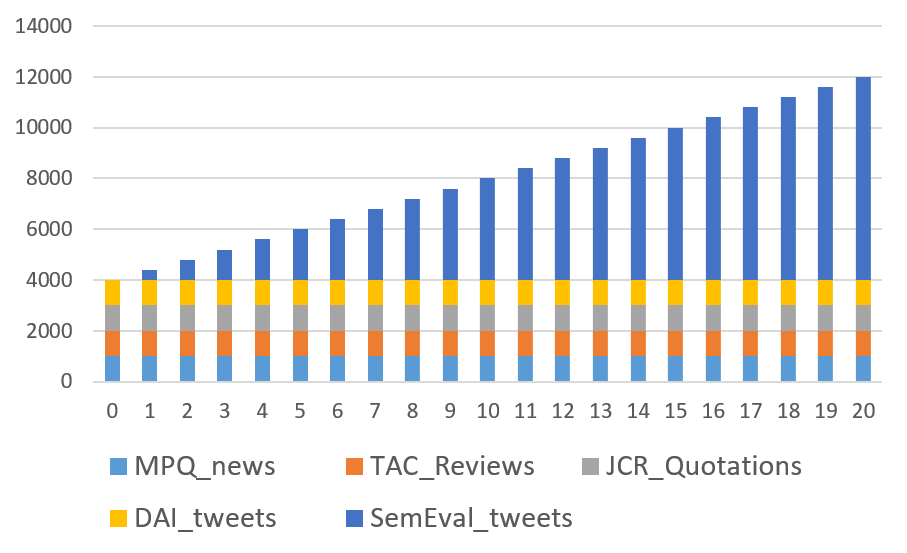
\includegraphics[width=0.49\textwidth]{img/methods/config_CrossDomain_SemEval_tweets.PNG}}
	\caption{Versuchsaufbau CrossDomain}
	\label{fig:Method_CrossDomain}
\end{figure}

Bei \ref{fig:Method_V6} ist die Zieldomäne SemEval\_tweets, die Vorgehensweise für die Zieldomäne MPQ\_news ist die Gleiche.
\subsection{Experiment SimilarDomain}
Im Experiment SimilarDomain wurde untersucht, wie stark sich die Performanz eines bereits trainierten CNN verbessert, wenn mit der Zieldomäne ähnlichen Daten weiter trainiert wird. Dazu wird zu beginn ein CNN mit 4000 Daten der Zieldomäne trainiert. Anschliessend wird in 11 Teilschritten mit jeweils 400 domänenähnliche Daten das Experiment wiederholt.
Domänenähnlich wird folgendermassen definiert, es gibt zwei verschiedene Kategorieren. Die eine Kategorie sind Volltexte und die Andere Kurznachrichten.
Der konkrete Versuchsaufbau für die beiden Zieldomänen MPQ\_news und SemEval\_tweets ist in der Abbildung \ref{fig:Method_SimilarDomain} ersichtlich.
\begin{figure}[H]
	\centering
	\subfigure[Zieldomäne MPQ\_news]{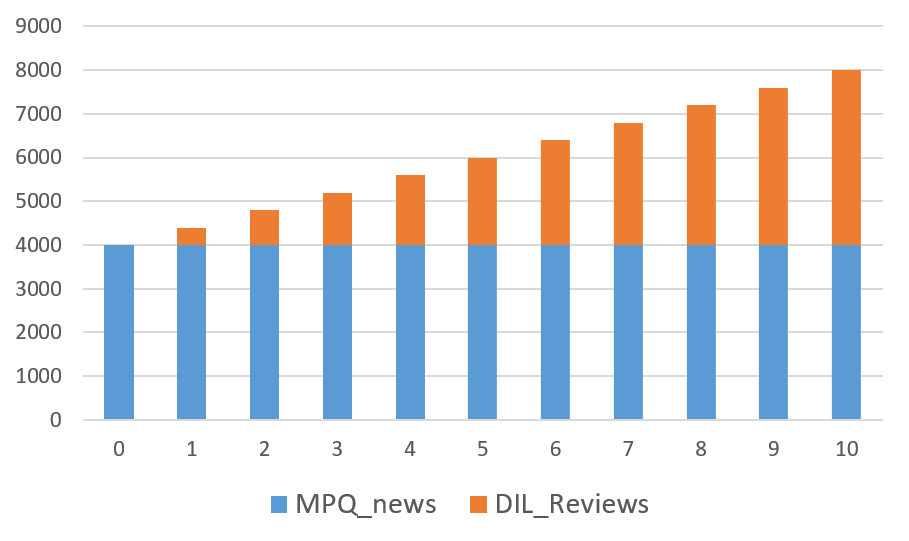
\includegraphics[width=0.49\textwidth]{img/methods/config_SimilarDomain_MPQ_news.PNG}}
	\subfigure[Zieldomäne SemEval\_tweets]{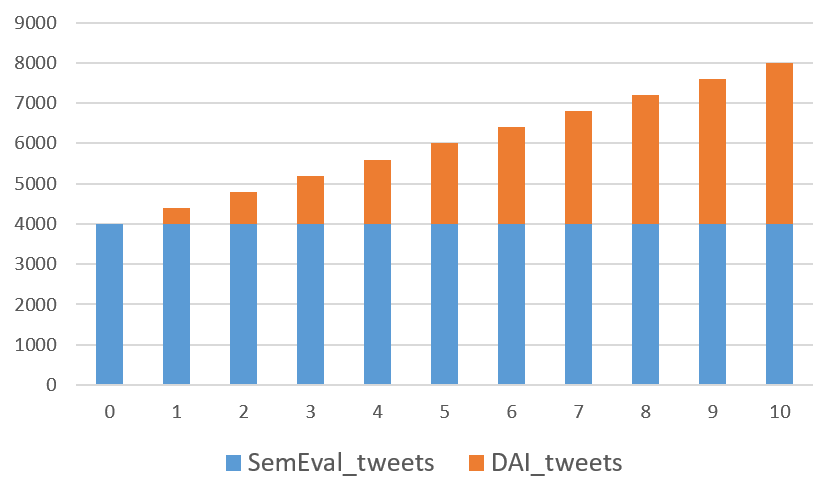
\includegraphics[width=0.49\textwidth]{img/methods/config_SimilarDomain_SemEval_tweets.PNG}}
	\caption{Versuchsaufbau SimilarDomain}
	\label{fig:Method_SimilarDomain}
\end{figure}

\subsection{Experiment BaseDomain}
\label{methods:v8}
Das Experiment BaseDomain dient als Baseline und somit Referenzwert für die Experimente CrossDomain und SimilarDomain.
Bei diesem Experiment wird nur mit den Daten der Zieldomäne trainiert und validiert \ref{fig:Method_BaseDomain}. Es dient als Anhaltspunkt, ob die Idee CrossDomain die Perfomanz des CNN effektiv erhöht.
\begin{figure}[H]
	\centering
	\subfigure[Zieldomäne MPQ\_news]{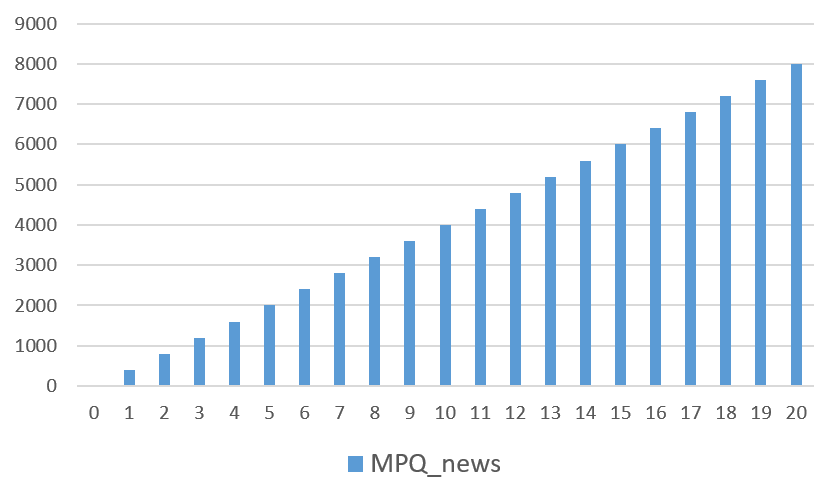
\includegraphics[width=0.49\textwidth]{img/methods/config_BaseDomain_MPQ_news.PNG}}
	\subfigure[Zieldomäne SemEval\_tweets]{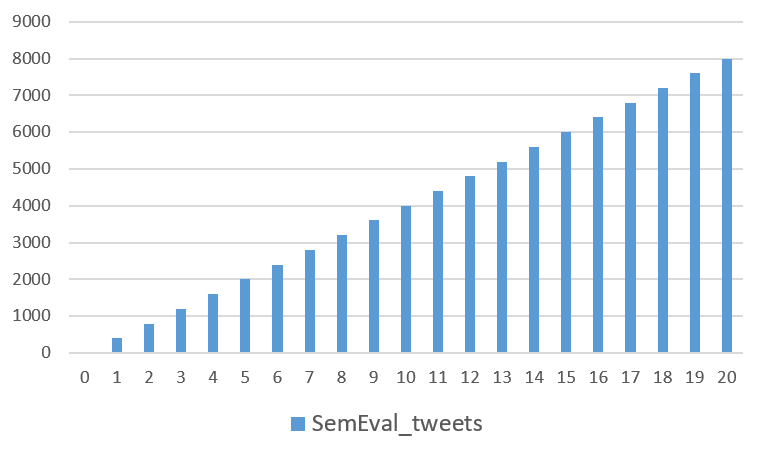
\includegraphics[width=0.49\textwidth]{img/methods/config_BaseDomain_SemEval_tweets.PNG}}
	\caption{Versuchsaufbau BaseDomain}
	\label{fig:Method_BaseDomain}
\end{figure}



